\hypertarget{ux4ebaux7c7bux793aux8303ux7684ux6570ux636eux7ed3ux6784ux4e0eux7cbeux786eux72b6ux6001ux91cdux5efa}{%
\section{人类示范的数据结构与精确状态重建}\label{ux4ebaux7c7bux793aux8303ux7684ux6570ux636eux7ed3ux6784ux4e0eux7cbeux786eux72b6ux6001ux91cdux5efa}}

\hypertarget{episode-ux5206ux5272ux4e0eux5408ux6cd5-transition}{%
\subsection{Episode 分割与合法 transition}\label{episode-ux5206ux5272ux4e0eux5408ux6cd5-transition}}

Minari 数据以 episode container 组织。每条人类示范名义 horizon 为 200，25 个 episode 共包含 5,000 个 source states；把每个 episode replay 得到的 final observation 计入 container 后共有 5,025 个 observations。合法 transition 只能在单个 episode 内连接相邻状态，因此数量是：

\[
\sum_{i=1}^{25}(T_i-1)=5000-25=4975.
\]

这里的减 25 来自每个 episode 最后状态没有同 episode 的下一状态，而不是把 24 个结束标记误读为只有 24 条 episode。实现同时尊重 episode container、\texttt{terminated}、\texttt{truncated/timeouts} 和文件 EOF；最终检查到的跨 episode transition 数为 0。

每个状态至少恢复 \texttt{qpos}、\texttt{qvel} 和 \texttt{desired\_orien}，再执行 MuJoCo forward，重新获得 low-dimensional observation、reward、success 和 RGB。恢复过程固定 XML、reward 类型、horizon、动作映射、renderer 和相机，避免把 legacy D4RL state 静默送入不兼容的新环境。

\hypertarget{ux673aux5668ux7cbeux5ea6ux6062ux590dux4e0eux4e00ux6b65-replay}{%
\subsection{机器精度恢复与一步 replay}\label{ux673aux5668ux7cbeux5ea6ux6062ux590dux4e0eux4e00ux6b65-replay}}

\begin{figure}
\centering
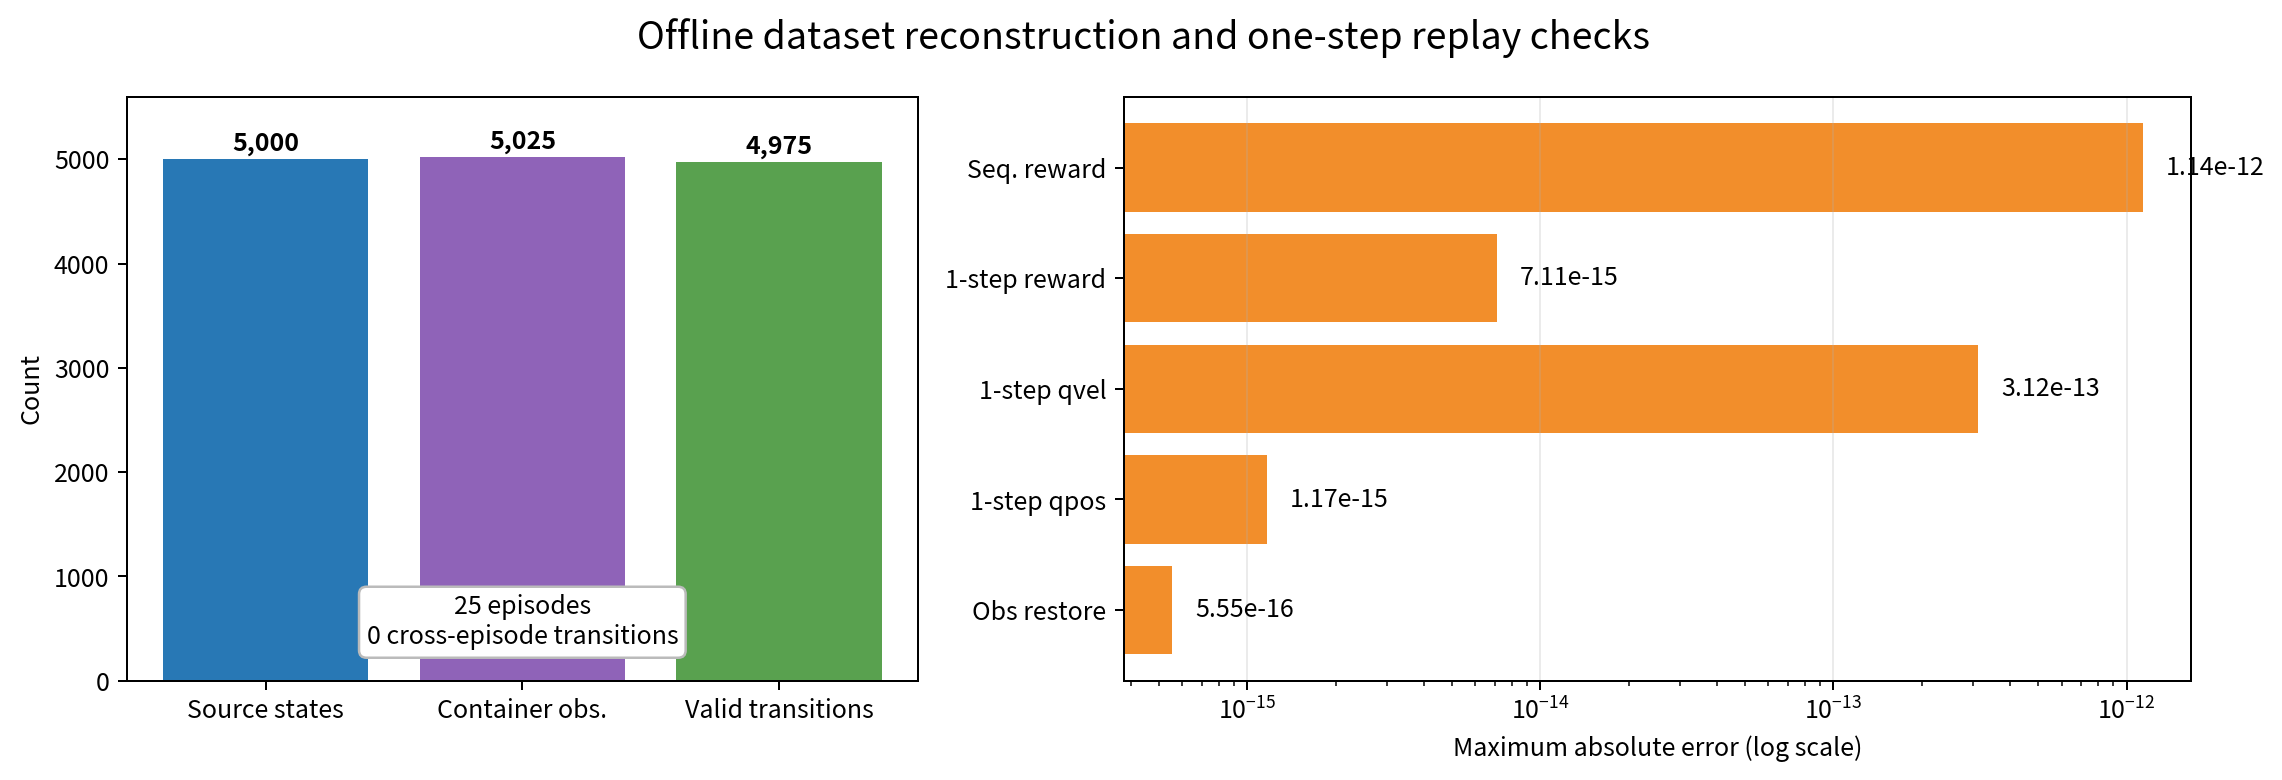
\includegraphics[width=\linewidth]{figures/03_reconstruction_validation.png}
\caption{数据重建和一步 replay 检查}
\end{figure}

\textbf{图 3｜数据重建与一步 replay。} 检查覆盖 25 episodes、100 个随机恢复状态和 32 个一步动力学样本。左图说明 5,000 source states、5,025 container observations 与 4,975 valid transitions 的关系；右图为最大绝对误差的对数坐标。该图是数据正确性验证，不是策略性能评测。

随机 100 个离线状态的 restored observation 最大绝对误差为 \texttt{5.551×10\^{}-16}。32 个从 \(s_t\) 执行数据动作 \(a_t\) 的一步 replay 中，qpos 最大误差为 \texttt{1.166×10\^{}-15}，qvel 为 \texttt{3.118×10\^{}-13}，reward 为 \texttt{7.105×10\^{}-15}。更长的顺序 replay 会积累浮点与仿真差异，observation 最大误差为 \texttt{2.265×10\^{}-2}，仍处于预先固定的 0.03 容差内；其 reward 最大误差为 \texttt{1.137×10\^{}-12}。同一 episode 中 \texttt{next\_rgb{[}t{]}} 与 \texttt{rgb{[}t+1{]}} 完全一致。

这些量并非文档装饰。若 \texttt{desired\_orien} 未恢复，策略看到的目标会错；若 final observation 或 timeout 处理错误，critic 会从下一条 episode bootstrap；若 action scaling 不一致，一步 replay 即使 observation 看起来接近，reward 与下一状态也会偏离。offline Q-learning 会反复放大这类系统性标签错误，所以在训练前将它们消除是后续结论成立的前提。

\hypertarget{rgbframe-stack-ux4e0eux5f52ux4e00ux5316}{%
\subsection{RGB、frame stack 与归一化}\label{rgbframe-stack-ux4e0eux5f52ux4e00ux5316}}

每个离线状态经过固定 MuJoCo renderer 得到 84×84 RGB。基础视觉策略使用 4-frame stack；frame stack 在 episode 开头按同一规则初始化，训练、闭环评测和状态恢复保持一致。hand qpos、hand qvel 和 previous action 与图像一起进入 actor，所有 normalization statistics 仅从训练 episode 计算。最终 E2 改用 8-step causal sequence，但没有改变相机、分辨率、动作边界或 Frozen Oracle controller。

RGB 重建的价值不仅是把状态``画成图片''。它把目标绿色笔、当前物体姿态和手物接触的可视信息与完全可 replay 的物理状态绑定起来，使后续可以在同一 episode 上生成视觉输入、privileged 监督和闭环结果，并能明确区分训练监督与部署输入。

\textbf{本章结论。} 数据管线恢复了 25 条 episode 和 4,975 条合法 transition，未产生跨 episode 连接；随机状态恢复和一步动力学 replay 达到机器精度。由此，后续 offline RL 与视觉蒸馏的主要误差可以归因于模型和闭环，而不是状态版本或数据边界错误。
